% !TeX root = ../../infdesc.tex
\section{Functions}
\secbegin{secFunctions}
\index{function|(}

One way of studying interactions between sets is by studying \textit{functions} between them, which we will define informally in \Cref{defFunction}. Functions are mathematical objects which assign to each element of one set exactly one element of another. Almost every branch of mathematics studies functions, be it directly or indirectly, and almost every application of mathematics arises from a translation of the abstract notion of a function to the real world. Just one example of this is the theory of computation---functions provide precisely the language necessary to describe the deterministic input-output behaviour of algorithms.

You might have come across the notion of a function before now. In schools, functions are often introduced as being like \textit{machines}---they have inputs and outputs, and on a given input they always return the same output. For instance, there is a function which takes integers as inputs and gives integers as outputs, which on the input $x$ returns the integer $x+3$.

This characterisation of functions, however, is clearly not precise enough for the purposes of mathematical proof. A next approximation to a precise definition of a function might look something like this:

\begin{definition}
\label{defFunction}
\index{function}
\index{domain}
\index{codomain}
\index{value!of a function}
\nindex{function}{$f : X \to Y$}{function}
\nindex{function value}{$f(x)$}{value of a function}
A \textbf{function} $f$ from a set $X$ to a set $Y$ is a specification of elements $f(x) \in Y$ for $x \in X$, such that
\[ \forall x \in X,\, \exists ! y \in Y,\, y = f(x) \]
Given $x \in X$, the (unique!) element $f(x) \in Y$ is called the \textbf{value} of $f$ at $x$.

The set $X$ is called the \textbf{domain} (or \textbf{source}) of $f$, and $Y$ is called the \textbf{codomain} (or \textbf{target}) of $f$. We write $f : X \to Y$ \inlatexnb{f :\ X \textbackslash{}to Y}\lindexmmc{to}{$\to$} to denote the assertion that $f$ is a function with domain $X$ and codomain $Y$.
\end{definition}

This is better---we're now talking about sets, and not mysterious `machines'.

Moreover, this definition establishes a close relationship between functions and the $\exists !$ quantifier: indeed, to say that $f$ assigns to each element of $X$ a unique element of $Y$ is to say precisely that
\[ \forall x \in X,\, \exists ! y \in Y,\, y = f(x) \]

Conversely, any true proposition of the form $\forall x \in X,\, \exists ! y \in Y,\, p(x,y)$ defines a function $f : X \to Y$: the function $f$ assigns to each $x \in X$ the unique $y \in Y$ such that $p(x,y)$ is true. In other words, $\forall x \in X,\, p(x,f(x))$ is true!

We can use this to generate some examples of functions.

\begin{example}
\label{exPositiveSquareRootFunction}
\Cref{exEveryPositiveRealHasUniqueSquareRoot} said that every positive real number has a unique positive square root; we proved this in \Cref{exEveryPositiveRealHasUniqueSquareRootProof}. What this means is that there is a function $r : (0, \infty) \to (0, \infty)$ defined by letting $r(x)$ be the (unique) positive square root of $x$, for each $x \in (0,\infty)$. That is, we have a function $r$ defined by $r(x)=\sqrt{x}$.
\end{example}

\begin{exercise}
Recall \Cref{exExamplesOfUniqueExistentialQuantifier}. Which of the statements (a), (b) or (c) is of the form $\forall x \in X,\, \exists ! y \in Y,\, p(x,y)$? For each statement of this form, determine the domain and codomain of the corresponding function, and write an expression defining this function.
\end{exercise}

\subsection*{Specifying a function}

Just like with sets, there are many ways to specify a function $f : X \to Y$, but when we do so, we must be careful that what we write really \textit{does} define a function!

This correctness of specification is known as \textit{well-definedness}, and ultimately amounts to verifying that the condition $\forall x \in X,\, \exists ! y \in Y,\, f(x)=y$ holds for the specification of $f$. Namely \textit{totality}, \textit{existence} and \textit{uniqueness}:
\begin{itemize}
\item \textbf{Totality.} A value $f(x)$ should be specified for each $x \in X$---this corresponds to the `$\forall x \in X$' quantifier in the definition of functions.
\item \textbf{Existence.} For each $x \in X$, the specified value $f(x)$ should actually exist, and should be an element of $Y$---this corresponds to the \textit{existence} part of the `$\exists ! y \in Y$' quantifier in the definition of functions.
\item \textbf{Uniqueness.} For each $x \in X$, the specified value $f(x)$ should refer to only one element of $Y$---this corresponds to the \textit{uniqueness} part of the `$\exists ! y \in Y$' quantifier in the definition of functions.
\end{itemize}

When specifying a function, you should justify each of these components of well-definedness unless they are extremely obvious. You will probably find that, in most cases, the only component in need of justification is uniqueness, but keep all three in mind.

\textbf{Lists.} If $X$ is finite, then we can specify a function $f : X \to Y$ by simply listing the values of $f$ at all possible elements $x \in X$. For example, we can define a function
\[ f : \{ 1, 2, 3 \} \to \{ \mathsf{red}, \mathsf{yellow}, \mathsf{green}, \mathsf{blue}, \mathsf{purple} \} \]
by declaring
\[ f(1) = \mathsf{red}, \quad f(2) = \mathsf{purple}, \quad f(3) = \mathsf{green} \]
Note that the function is at this point completely specified: we know its values at all elements of the domain $\{ 1, 2, 3 \}$. It doesn't matter that some of the elements of the codomain ($\mathsf{yellow}$ and $\mathsf{blue}$) are unaccounted for---all that matters is that each element of the domain is associated with exactly one element of the codomain.

Unfortunately, most of the sets that we work with will be infinite, or of an unspecified finite size; in these cases, simply writing a list of values isn't sufficient. Fortunately for us, there are other ways of specifying functions.

\textbf{Formulae.} In many cases, particularly when the domain $X$ and codomain $Y$ are number sets, we can define a function by giving a formula for the value of $f(x)$ for each $x \in X$. For example, we can define a function $f : \mathbb{R} \to \mathbb{R}$ by letting
\[ f(x) = x^2 + 3 \text{ for all } x \in \mathbb{R} \]

\textbf{By cases.} It will at times be convenient to define a function using different specifications for different elements of the domain.  A very simple example is the \textit{absolute value function} $|{-}| : \mathbb{R} \to \mathbb{R}$, defined for $x \in \mathbb{R}$
\[ |x| = \begin{cases} x & \text{if } x \ge 0 \\ -x & \text{if } x \le 0 \end{cases} \]
Here we have split into two cases based on the conditions $x \ge 0$ and $x \le 0$.

When specifying a function $f : X \to Y$ by cases, it is important that the conditions be:
\begin{itemize}
\item \textbf{exhaustive}: given $x \in X$, at least one of the conditions on $X$ must hold; and
\item \textbf{compatible}: if any $x \in X$ satisfies more than one condition, the specified value must be the same no matter which condition is picked.
\end{itemize}

For the absolute value function defined above, these conditions are satisfied. Indeed, for $x \in \mathbb{R}$, it is certainly the case that $x \ge 0$ or $x \le 0$, so the conditions are exhaustive. Moreover, given $x \in \mathbb{R}$, if both $x \ge 0$ and $x \le 0$, then $x=0$---so we need to check that the specification yields the same value when $x=0$ regardless of which condition we pick. The $x \ge 0$ condition yields the value $0$, and the $x \le 0$ condition yields the value $-0$, which is equal to $0$---so the conditions are compatible. We could have used $x<0$ instead of $x \le 0$; in this case the conditions are \textit{mutually exclusive}, so certainly compatible because they do not overlap.

\textbf{Algorithms.} You might, on first exposure to functions, have been taught to think of a function as a \textit{machine} which, when given an \textit{input}, produces an \textit{output}. This `machine' is defined by saying what the possible inputs and outputs are, and then providing a list of instructions (an \textit{algorithm}) for the machine to follow, which on any input produces an output---and, moreover, if fed the same input, the machine always produces the same output. 

For example, we might instruct a machine to take rational numbers as inputs and give rational numbers as outputs, and to follow the following sequence of steps on a given input
\begin{center}
\label{txtAlgorithmicallyDefinedFunctionExample}
multiply by $2$ $\to$ add $5$ $\to$ square the result $\to$ divide by $6$
\end{center}
This `machine' defines a function $M : \mathbb{Q} \to \mathbb{Q}$ which, in equation form, is specified by
\[ M(x) = \frac{(2x+5)^2}{6} \text{ for all } x \in \mathbb{Q} \]
In our more formal set-up, therefore, we can define a function $M : I \to O$ by specifying:
\begin{itemize}
\item a set $I$ of all \textbf{inputs};
\item a set $O$ of potential \textbf{outputs}; and
\item a deterministic\footnote{The word `deterministic' just means that the algorithm always produces the same output on a single input.} algorithm which describes how an input $x \in I$ is transformed into an output $M(x) \in O$.
\end{itemize}
That is, the domain is the set $I$ of all possible `inputs', the codomain is a set $O$ containing all the possible `outputs', and the function $M$ is a rule specifying how an input is associated with the corresponding output.

For now, we will use algorithmic specifications of functions only sparingly---this is because it is much harder to make formal what is meant by an `algorithm', and it is important to check that a given algorithm is deterministic.

\subsection*{Function equality}

In \Cref{secSets} we discussed how there may be many different possible ways of characterising equality of sets. This matter was resolved by declaring that two sets are equal if and only if they have the same elements (this was \Cref{axSetEquality}).

A similar matter arises for functions. For example, consider the function $f : \mathbb{R} \to \mathbb{R}$ defined by $f(x) = 2x$ for all $x \in \mathbb{R}$, and the function $g : \mathbb{R} \to \mathbb{R}$, defined by letting $g(x)$ be the result of taking $x$, multiplying it by three, dividing the result by four, dividing the result by six, and then multiplying the result by sixteen. It so happens that $g(x) = 2x$ for all $x \in \mathbb{R}$ as well, but that is not how $g$ is defined; moreover, if $f$ and $g$ were implemented as algorithms, then it would take longer to compute the values of $g$ than it would take to compute the values of $f$.

Should we consider $f$ and $g$ to be \textit{equal}? If we are only interested in whether $f$ and $g$ have the same values on each argument, then the answer should be `yes'; if we are interested in the algorithmic behaviour of $f$ and $g$, then the answer should be `no'.

We resolve this dilemma with the following axiom. By adopting this axiom, we are stating that the functions $f$ and $g$ discussed above are equal.

\begin{axiom}[Function extensionality]
\label{axFunctionExtensionality}
Let $f : X \to Y$ and $g : A \to B$ be functions. Then $f = g$ if and only if the following conditions hold:
\begin{enumerate}[(i)]
\item $X=A$ and $Y=B$; and
\item $f(x) = g(x)$ for all $x \in X$.
\end{enumerate}
\end{axiom}

\begin{strategy}[Proving two functions are equal]
\label{strFunctionExtensionality}
Given functions $f, g : X \to Y$ with the same domain and codomain, in order to prove that $f=g$, it suffices to prove that $f(x) = g(x)$ for all $x \in X$.
\end{strategy}

A consequence of \Cref{axFunctionExtensionality} is that, for fixed sets $X$ and $Y$, a function $X \to Y$ is uniquely determined by its input-output pairs. This set is called the \textit{graph} of the function; the proof of the equivalence between functions and their graphs is the content of \Cref{thmFunctionsAsGraphs}.

\begin{definition}
\label{defFunctionGraph}
\index{graph!of a function}
Let $f : X \to Y$ be a function. The \textbf{graph} of $f$ is the subset $\mathrm{Gr}(f) \subseteq X \times Y$ \inlatex{mathrm\{Gr\}}\lindexmmc{mathrm}{$\mathrm{Aa}, \mathrm{Bb}, \dots$} defined by
\[ \mathrm{Gr}(f) = \{ (x, f(x)) \mid x \in X \} = \{ (x,y) \in X \times Y \mid y=f(x) \} \]
\end{definition}

\begin{example}
\label{exGraphsOfFunctionsRToR}
Given a (sufficiently well-behaved) function $f : \mathbb{R} \to \mathbb{R}$, we can represent $\mathrm{Gr}(f) \subseteq \mathbb{R} \times \mathbb{R}$ by plotting it on a pair of axes using Cartesian coordinates in the usual way. For example, if $f$ is defined by $f(x)=\frac{x}{2}$ for all $x \in \mathbb{R}$, then its graph
\[ \mathrm{Gr}(f) = \left\{ \left( x, \frac{x}{2} \right) \ \bigg|\ x \in \mathbb{R} \right\} \]\nindex{graph}{$\mathrm{Gr}(f)$}{graph of a function}
can be represented by graph plot in \Cref{figGraphOfXOverTwo}.

\begin{figure}[H]
\centering
\fitwidthc{0.9}{\begin{tikzpicture}
\draw[-latex] (-7.3, 0) -- (7.3, 0) node[right] {$x$} ;
\draw[-latex] (0, -3.8) -- (0, 3.8) node[above] {$y$} ;
\foreach \i in {-7,-6,-5,-4,-3,-2,-1,1,2,3,4,5,6,7} {
    \draw[lightgray] (\i, -3.8) -- (\i, 3.8) ;
    \draw (\i, 0) -- (\i, -0.1) node[below, fill=white] {$\i$} ;
}
\foreach \i in {-3,-2,-1,1,2,3} {
    \draw[lightgray] (-7.3, \i) -- (7.3, \i) ;
    \draw (0, \i) -- (-0.1, \i) node[left, fill=white] {$\i$} ;
}
\draw[blue] (-7.2, -3.6) -- (7.2, 3.6) ;
\draw[blue] (4.2, 2.1) node[above left, fill=white] {$y=\dfrac{x}{2}$} ;
\end{tikzpicture}}
\caption{Graph of the function $f : \mathbb{R} \to \mathbb{R}$ defined by $f(x) = \frac{x}{2}$ for all $x \in \mathbb{R}$}
\label{figGraphOfXOverTwo}
\end{figure}
\end{example}

\begin{exercise}
Find a function $f : \mathbb{Z} \to \mathbb{Z}$ whose graph is equal to the set
\[ \{ \dots, ({-2}, {-5}), ({-1}, {-2}), (0, 1), (1, 4), (2, 7), (3, 10), \dots \} \]
\end{exercise}

\Cref{thmFunctionsAsGraphs} below provides a way of verifying that a function is well-defined by characterising their graphs.

\begin{theorem}
\label{thmFunctionsAsGraphs}
Let $X$ and $Y$ be sets. A subset $G \subseteq X \times Y$ is the graph of a function if and only if
\[ \forall x \in X,\, \exists ! y \in Y,\, (x,y) \in G \]
\end{theorem}
\begin{cproof}
($\Rightarrow$). Suppose $G \subseteq X \times Y$ is the graph of a function, say $G = \mathrm{Gr}(f)$ for some $f : X \to Y$. Then for each $x \in X$, it follows from well-definedness of $f$ that $f(x)$ is the unique element $y \in Y$ for which $(x, y) \in G$. That is, $(x,f(x)) \in G$, and if $y \in Y$ with $(x,y) \in G$, then $y=f(x)$.

($\Leftarrow$). Suppose $G \subseteq X \times Y$ satisfies $\forall x \in X,\, \exists ! y \in Y,\, (x,y) \in G$. Define a function $f : X \to Y$ by, for each $x \in X$, defining the value $f(x)$ to be the unique element $y \in Y$ for which $(x,y) \in G$. Well-definedness of $f$ is then immediate from our assumption of the existence and uniqueness of such a value of $y$ for each $x \in X$.
\end{cproof}

\begin{example}
The set $G$ defined by
\[ G = \{ (1, \mathsf{red}), (2, \mathsf{red}), (3, \mathsf{green}) \} \]
is the graph of a function $f : \{ 1, 2, 3 \} \to \{ \mathsf{red}, \mathsf{green}, \mathsf{blue} \}$. The function $f$ is defined by
\[ f(1) = \mathsf{red}, \quad f(2) = \mathsf{red}, \quad f(3) = \mathsf{green} \]
However, $G$ is \textit{not} the graph of a function $\{ 1, 2, 3, 4 \} \to \{ \mathsf{red}, \mathsf{green}, \mathsf{blue} \}$, since $G$ contains no elements of the form $(4,y)$ for $y \in \{ \mathsf{red}, \mathsf{green}, \mathsf{blue} \}$. Moreover, the set $G'$ defined by
\[ G' = \{ (1, \mathsf{red}), (2, \mathsf{red}), (2, \mathsf{blue}), (3, \mathsf{green}) \} \]
does not define the graph of a function $\{ 1, 2, 3 \} \to \{ \mathsf{red}, \mathsf{green}, \mathsf{blue} \}$, since there is not a \textit{unique} element of the form $(2,y)$ in $G'$---rather, there are two of them!
\end{example}

\begin{exercise}
For each of the following specifications of sets $X$, $Y$, $G$, determine whether or not $G$ is the graph of a function from $X$ to $Y$.
\begin{enumerate}[(a)]
\item $X = \mathbb{R}$, $Y = \mathbb{R}$, $G = \{ (a, a^2) \mid a \in \mathbb{R} \}$;
\item $X = \mathbb{R}$, $Y = \mathbb{R}$, $G = \{ (a^2, a) \mid a \in \mathbb{R} \}$;
\item $X = [0, \infty)$, $Y = [0, \infty)$, $G = \{ (a^2, a) \mid a \in [0, \infty) \}$;
\item $X = \mathbb{Q}$, $Y = \mathbb{Q}$, $G = \{ (x, y) \in \mathbb{Q} \times \mathbb{Q} \mid xy = 1 \}$.
\item $X = \mathbb{Q}$, $Y = \mathbb{Q}$, $G = \{ (a, a) \mid a \in \mathbb{Z} \}$;
\end{enumerate}
\end{exercise}

\begin{aside}
In light of \Cref{thmFunctionsAsGraphs}, some people choose to define functions $X \to Y$ as particular subsets of $X \times Y$---that is, they identify functions with their graphs. This is particularly useful when studying the logical foundations of mathematics. We avoid this practice here, because it is not conceptually necessary, and it would preclude other possible ways of encoding functions.
\end{aside}

There is a class of functions called \textit{identity functions} that, despite being very simple, are so important that we will give them a numbered definition!

\begin{definition}
\label{defIdentityFunction}
\index{function!identity}
\index{identity function}
Let $X$ be a set. The \textbf{identity function} on $X$ is the function $\mathrm{id}_X : X \to X$\nindex{idX}{$\mathrm{id}_X$}{identity function} \inlatex{mathrm\{id\}\_X}\lindexmmc{mathrm}{$\mathrm{Aa}, \mathrm{Bb}, \dots$} defined by $\mathrm{id}_X(x)=x$ for all $x \in X$.
\end{definition}

You should convince yourself that the specification of $\mathrm{id}_X$ given in \Cref{defIdentityFunction} is well-defined.

Another interesting example of a function is the \textit{empty function}, which is useful in coming up with counterexamples and proving combinatorial identities (see \Cref{secCountingPrinciples}).

\begin{definition}
\label{defEmptyFunction}
\index{function!empty}
\index{empty function}
Let $X$ be a set. The \textbf{empty function} with codomain $X$ is the (unique!) function $\varnothing \to X$. It has no values, since there are no elements of its domain.
\end{definition}

Again, you should convince yourself that this specification is well-defined. Conceptually, convincing yourself of this is not easy; but writing down the proof of well-definedness is extremely easy---you will find that there is simply nothing to prove!

\begin{example}
Define $f : \mathbb{R} \to \mathbb{R}$ by the equation $f(x)^2=x$ for all $x \in \mathbb{R}$. This is not well-defined for a few reasons. First, if $x<0$ then there is no real number $y$ such that $y^2=x$, so for $x<0$ there are no possible values of $f(x)$ in the codomain of $f$, so \textit{existence} fails. Second, if $x>0$ then there are in fact \textit{two} real numbers $y$ such that $y^2=x$, namely the positive square root $\sqrt{x}$ and the negative square root $-\sqrt{x}$. The specification of $f$ does not indicate which of these values to take, so \textit{uniqueness} fails.

Notice that the function $r : (0, \infty) \to (0, \infty)$ from \Cref{exPositiveSquareRootFunction} \textit{is} (well-)defined by the equation $r(x)^2 = x$ for all $x \in (0, \infty)$. This illustrates why it is very important to specify the domain and codomain when defining a function.
\end{example}

\begin{exercise}
Which of the following specifications of functions are well-defined?
\begin{enumerate}[(a)]
\item $g : \mathbb{Q} \to \mathbb{Q}$ defined by the equation $(x+1)g(x)=1$ for all $x \in \mathbb{Q}$;
\item $h : \mathbb{N} \to \mathbb{Q}$ defined by $(x+1)h(x)=1$ for all $x \in \mathbb{N}$;
\item $k : \mathbb{N} \to \mathbb{N}$ defined by $(x+1)k(x)=1$ for all $x \in \mathbb{N}$;
\item $\ell : \mathbb{N} \to \mathbb{N}$ defined by $\ell(x)=\ell(x)$ for all $x \in \mathbb{N}$.
\end{enumerate}
\end{exercise}

\begin{exercise}
\label{exWellDefinednessOfFunctionOnUnion}
Find a condition on sets $X$ and $Y$ such that the specification of a function $i : X \cup Y \to \{ 0, 1 \}$ given by
\[ i(z) = \begin{cases} 0 & \text{if } z \in X \\ 1 & \text{if } z \in Y \end{cases} \]
to be well-defined.
\begin{backhint}
\hintref{exWellDefinednessOfFunctionOnUnion}
What is the value of $i(z)$ if $z \in X \cap Y$?
\end{backhint}
\end{exercise}

\subsection*{Composition of functions}

In our section on sets, we talked about various operations that can be performed on sets---union, intersection, and so on. There are also operations on functions, by far the most important of which is \textit{composition}. To understand how composition works, let's revisit the algorithmically defined function $M : \mathbb{Q} \to \mathbb{Q}$ from page \pageref{txtAlgorithmicallyDefinedFunctionExample}:
\begin{center}
multiply by $2$ $\to$ add $5$ $\to$ square the result $\to$ divide by $6$
\end{center}
The function $M$ is, in some sense, a \textit{sequence} of functions, performed one-by-one until the desired result is reached. This is precisely \textit{composition of functions}.

\begin{definition}
\label{defComposition}
\label{defComposite}
\index{composite}
\index{function!composition}
Let $f : X \to Y$ and $g : Y \to Z$ be functions. The \textbf{composite} of $f$ and $g$ is the function $g \circ f : X \to Z$%
\nindex{composition}{$\circ$}{composition} \inlatexnb{g \textbackslash{}circ f}\lindexmmc{circ}{$\circ$} (read `$g$ composed with $f$' or `$g$ after $f$' or even just `$g$ $f$') defined by
\[ (g \circ f)(x) = g(f(x)) \text{ for all } x \in X \]
\end{definition}
Intuitively, $g \circ f$ is the function resulting from first applying $f$, and then applying $g$, to the given input.

\begin{commonerror}
Function composition is in some sense written `backwards': in the expression $g \circ f$, the function which is applied \textit{first} is written \textit{last}---there is a good reason for this: the argument to the function is written after the function! However, this mis-match often trips students up on their first exposure to function composition, so be careful!
\end{commonerror}

\begin{example}
\label{exDecompositionOfFunctionQToQ}
The function $M$ from page \pageref{txtAlgorithmicallyDefinedFunctionExample} can be defined as the composite
\[ M = ((k \circ h) \circ g) \circ f \]
where
\begin{itemize}
\item $f : \mathbb{Q} \to \mathbb{Q}$ is defined by $f(x)=2x$ for all $x \in \mathbb{Q}$;
\item $g : \mathbb{Q} \to \mathbb{Q}$ is defined by $g(x)=x+5$ for all $x \in \mathbb{Q}$;
\item $h : \mathbb{Q} \to \mathbb{Q}$ is defined by $h(x)=x^2$ for all $x \in \mathbb{Q}$;
\item $k : \mathbb{Q} \to \mathbb{Q}$ is defined by $k(x)=\frac{x}{6}$ for all $x \in \mathbb{Q}$.
\end{itemize}
\end{example}

\begin{exercise}
Let $f,g,h,k : \mathbb{Q} \to \mathbb{Q}$ be as in \Cref{exDecompositionOfFunctionQToQ}. Compute equations defining the following composites:
\begin{enumerate}[(a)]
\item $f \circ g$;
\item $g \circ f$;
\item $((f \circ g) \circ h) \circ k$;
\item $f \circ (g \circ (h \circ k))$;
\item $(g \circ g) \circ (g \circ g)$.
\end{enumerate}
\end{exercise}

\begin{example}
\label{exCompositionWithIdentityIsTrivial}
Let $f : X \to Y$ be any function. Then
\[ \mathrm{id}_Y \circ f = f = f \circ \mathrm{id}_X \]
To see this, let $x \in X$. Then
\begin{align*}
(\mathrm{id}_Y \circ f)(x) &= \mathrm{id}_Y(f(x)) && \text{by definition of composition} \\
&= f(x) && \text{by definition of $\mathrm{id}_Y$} \\
&= f(\mathrm{id}_X(x)) && \text{by definition of $\mathrm{id}_X$} \\
&= (f \circ \mathrm{id}_X)(x) && \text{by definition of composition}
\end{align*}
Equality of the three functions in question follows.
\end{example}

\begin{exercise}
\label{exCompositionIsAssociative}
Prove that composition of functions is \textit{associative}, that is, if $f : X \to Y$, $g : Y \to Z$ and $h : Z \to W$ are functions, then
\[ h \circ (g \circ f) = (h \circ g) \circ f : X \to W \]
As a consequence of associativity, when we want to compose more than two functions, it doesn't matter what order we compose the functions in. As such, we can just write $h \circ g \circ f$.
\end{exercise}

\begin{exercise}
\label{exCompositionWithoutMatchingCodomains}
Let $f : X \to Y$ and $g : Z \to W$ be functions, and suppose that $Y \subsetneqq Z$. Note that there is a function $h : X \to W$ defined by $h(x)=g(f(x))$ for all $x \in X$. Write $h$ as a composite of functions involving $f$ and $g$.
\begin{backhint}
\hintref{exCompositionWithoutMatchingCodomains}
Look closely at \Cref{defComposition}.
\end{backhint}
\end{exercise}

\subsection*{Characteristic functions}

A class of functions that are particularly useful for proving results about sets are \textit{characteristic functions}.

\begin{definition}
\label{defCharacteristicFunction}
\index{characteristic function}
\index{function!characteristic}
Let $X$ be a set and let $U \subseteq X$. The \textbf{characteristic function} of $U$ is the function $\chi_U : X \to [2]$ \inlatex{chi\_\{U\}}, where $[2] = \{ 0, 1 \}$ (see \Cref{defBracketN}), defined by
\[ \chi_U(a) = \begin{cases} 1 & \text{if } a \in U \\ 0 & \text{if } a \not\in U \end{cases} \]
\end{definition}

\begin{example}
Consider the subset $U = \{ 1,3,5 \} \subseteq [6]$. Then the values of the characteristic function $\chi_U : [6] \to [2]$ are given by
\[ \begin{matrix} \chi_U(1) = 1 & \chi_U(2) = 0 & \chi_U(3) = 1 \\ \chi_U(4) = 0 & \chi_U(5) = 1 & \chi_U(6) = 0 \end{matrix} \]
\end{example}

\begin{theorem}
\label{thmCharacteristicFunctionsCharacteriseSubsets}
Let $X$ be a set and let $U, V \subseteq X$. Then $U=V$ if and only if $\chi_U = \chi_V$.
\end{theorem}

\begin{cproof}
\fixlistskip
\begin{itemize}
\item ($\Rightarrow$)
%% BEGIN EXTRACT (xtrAssumeExample) %%
Assume $U=V$ and let $a \in X$. Then
\begin{align*}
\chi_U(a) = 1 & \Leftrightarrow a \in U && \text{by definition of $\chi_U$} \\
&\Leftrightarrow a \in V && \text{since $U=V$} \\
&\Leftrightarrow \chi_V(a) = 1 && \text{by definition of $\chi_V$}
\end{align*}
%% END EXTRACT %%
Likewise $\chi_U(a) = 0$ if and only if $\chi_V(a) = 0$, so that $\chi_U = \chi_V$ by function extensionality.

\item ($\Leftarrow$) Assume $\chi_U = \chi_V$ and let $a \in X$. Then
\begin{align*}
a \in U & \Leftrightarrow \chi_U(a) = 1 && \text{by definition of $\chi_U$} \\
&\Leftrightarrow \chi_V(a) = 1 && \text{since $\chi_U = \chi_V$} \\
&\Leftrightarrow a \in V && \text{by definition of $\chi_V$}
\end{align*}
so $U=V$ by set extensionality.
\end{itemize}
\end{cproof}

\begin{strategy}[Proving set identities using characteristic functions]
\label{strSetIdentitiesFromCharacteristicFunctions}
In order to prove that two subsets $U$ and $V$ of a set $X$ are equal, it suffices to prove that $\chi_U = \chi_V$.
\end{strategy}

\begin{theorem}
\label{thmSetIdentitiesFromCharacteristicFunctions}
Let $X$ be a set and let $U,V \subseteq X$. Then
\begin{enumerate}[(a)]
\item $\chi_{U \cap V}(a) = \chi_U(a) \chi_V(a)$ for all $a \in X$;
\item $\chi_{U \cup V}(a) = \chi_U(a) + \chi_V(a) - \chi_U(a)\chi_V(a)$ for all $a \in X$;
\item $\chi_{X \setminus U}(a) = 1 - \chi_U(a)$ for all $a \in X$.
\end{enumerate}
\end{theorem}

\begin{cproof}[of {(a)}]
Let $a \in X$. Since the only values that $\chi_U(a)$ and $\chi_V(a)$ can take are $0$ and $1$, we have
\[ \chi_U(a) \chi_V(a) = \begin{cases} 1 & \text{if $\chi_U(a) = 1$ and $\chi_V(a) = 1$} \\ 0 & \text{otherwise} \end{cases} \]
But $\chi_U(a) = 1$ if and only if $a \in U$ and $\chi_V(a) = 1$ if and only if $a \in V$, so that
\[ \chi_U(a) \chi_V(a) = \begin{cases} 1 & \text{if $a \in U \cap V$} \\ 0 & \text{if $a \not\in U \cap V$} \end{cases} \]
This is exactly to say that $\chi_U(a) \chi_V(a) = \chi_{U \cap V}(a)$, as required.
\end{cproof}

\begin{exercise}
Prove parts (b) and (c) of \Cref{thmSetIdentitiesFromCharacteristicFunctions}.
\end{exercise}

\Cref{thmSetIdentitiesFromCharacteristicFunctions} can be used in conjunction with \Cref{strSetIdentitiesFromCharacteristicFunctions} to prove set theoretic identities using their characteristic functions.

\begin{example}
In \Cref{exIntersectionDistributesOverUnion} we proved that $X \cap (Y \cup Z) = (X \cap Y) \cup (X \cap Z)$ for all sets $X$, $Y$ and $Z$. We prove this again using characteristic functions, considering $X$, $Y$ and $Z$ as subsets of a universal set $\mathcal{U}$.

So let $a \in U$. Then
\begin{align*}
& \chi_{X \cap (Y \cup Z)}(a) && \\
&= \chi_X(a) \chi_{Y \cup Z}(a) && \text{by \Cref{thmSetIdentitiesFromCharacteristicFunctions}(a)} \\
&= \chi_X(a) (\chi_Y(a) + \chi_Z(a) - \chi_Y(a)\chi_Z(a)) && \text{by \Cref{thmSetIdentitiesFromCharacteristicFunctions}(b)} \\
&= \chi_X(a)\chi_Y(a) + \chi_X(a)\chi_Z(a) - \chi_X(a)\chi_Y(a)\chi_Z(a) && \text{rearranging} \\
&= \chi_X(a)\chi_Y(a) + \chi_X(a)\chi_Z(a) - \chi_X(a)^2\chi_Y(a)\chi_Z(a) && \text{since $\chi_X(a)^2=\chi_X(a)$} \\
&= \chi_{X \cap Y}(a) + \chi_{X \cap Z}(a) - \chi_{X \cap Y}(a) \chi_{X \cap Z}(a) && \text{by \Cref{thmSetIdentitiesFromCharacteristicFunctions}(a)} \\
&= \chi_{(X \cap Y) \cup (X \cap Z)}(a) && \text{by \Cref{thmSetIdentitiesFromCharacteristicFunctions}(b)}
\end{align*}
Using \Cref{strSetIdentitiesFromCharacteristicFunctions}, it follows that $X \cap (Y \cup Z) = (X \cap Y) \cup (X \cap Z)$.
\end{example}

\begin{exercise}
Use characteristic functions to prove de Morgan's laws for pairwise unions and intersections (\Cref{thmDeMorganForSets}).
\end{exercise}

\subsection*{Images and preimages}

\begin{definition}
\label{defImage}
Let $f : X \to Y$ be a function and let $U \subseteq X$. The \textbf{image of} $U$ \textbf{under} $f$ is the subset $f[U] \subseteq Y$\nindex{functionImage}{$f[U]$}{image} (also written $f_*(U)$ \inlatexnb{f\_*} or even just $f(U)$) is defined by
\[ f[U] = \{ f(x) \mid x \in U \} = \{ y \in Y \mid \exists x \in U,\, y = f(x) \} \]
That is, $f[U]$ is the set of values that the function $f$ takes when given inputs from $U$.

The \textbf{image of} $f$ is the image of the entire domain, i.e.\ the set $f[X]$.
\end{definition}

\begin{example}
Let $f : \mathbb{R} \to \mathbb{R}$ be defined by $f(x)=x^2$. The image of $f$ is the set $[0,\infty)$ of all nonnegative real numbers. Let's prove this:
\begin{itemize}
\item ($f[\mathbb{R}] \subseteq [0,\infty)$). Let $y \in f[\mathbb{R}]$. Then $y=x^2$ for some $x \in \mathbb{R}$. But $x^2 \ge 0$, so we must have $y \in [0,\infty)$, as required.
\item ($[0,\infty) \subseteq f[\mathbb{R}]$). Let $y \in [0,\infty)$. Then $\sqrt{y} \in \mathbb{R}$, and $y = (\sqrt{y})^2 = f(\sqrt{y})$. Hence $y \in f[\mathbb{R}]$, as required.
\end{itemize}
We have shown by double containment that $f[\mathbb{R}] = [0,\infty)$.
\end{example}

\begin{exercise}
For each of the following functions $f$ and subsets $U$ of their domain, describe the image $f[U]$.
\begin{enumerate}[(a)]
\item $f : \mathbb{Z} \to \mathbb{Z}$ defined by $f(n)=3n$, with $U = \mathbb{N}$;
\item $f : X \to X \times X$ (where $X$ is any set) defined by $f(x)=(x,x)$ with $U=X$;
\item $f : \{ a, b, c \} \to \{ 1, 2, 3 \}$ defined by $f(a)=1$, $f(b)=3$ and $f(c)=1$, with $U=\{a,b,c\}$.
\end{enumerate}
\end{exercise}

\begin{exercise}
Prove that $f[\varnothing] = \varnothing$ for all functions $f$.
\end{exercise}

\begin{example}
\label{exImageOfIntersectionSubsetIntersectionOfImage}
Let $f : X \to Y$ be a function and let $U, V \subseteq X$. Then $f[U \cap V] \subseteq f[U] \cap f[V]$. To see this, let $y \in f[U \cap V]$. Then $y = f(x)$ for some $x \in U \cap V$. By definition of intersection, $x \in U$ and $x \in V$. Since $x \in U$ and $y=f(x)$, we have $y \in f[U]$; likewise, since $x \in V$, we have $y \in f[V]$. But then by definition of intersection, we have $y \in f[U] \cap f[V]$.
\end{example}

\begin{exercise}
Let $f : X \to Y$ be a function and let $U, V \subseteq X$. We saw in \Cref{exImageOfIntersectionSubsetIntersectionOfImage} that $f[U \cap V] \subseteq f[U] \cap f[V]$. Determine which of the following is true, and for each, provide a proof of its truth or falsity:
\begin{enumerate}[(a)]
\item $f[U] \cap f[V] \subseteq f[U \cap V]$;
\item $f[U \cup V] \subseteq f[U] \cup f[V]$;
\item $f[U] \cup f[V] \subseteq f[U \cup V]$.
\end{enumerate}
\end{exercise}

\begin{definition}
\label{defPreimage}
Let $f : X \to Y$ be a function and let $V \subseteq Y$. The \textbf{preimage of} $V$ \textbf{under} $f$ is the subset $f^{-1}[V]$\nindex{functionPreImage}{$f^{-1}[V]$}{preimage} \inlatexnb{f\^{}\{-1\}} (also written $f^*(V)$ \inlatexnb{f\^{}*}, or just $f^{-1}(V)$) is defined by
\[ f^{-1}[V] = \{ x \in X \mid f(x) \in V \} = \{ x \in X \mid \exists y \in V,\, f(x) = y \} \]
That is, $f^{-1}[V]$ is the set of all the elements of its domain $X$ that the function $f$ sends to elements of $V$.
\end{definition}

\begin{example}
Let $f : \mathbb{Z} \to \mathbb{Z}$ be the function defined by $f(x)=x^2$ for all $x \in X$. Then
\begin{itemize}
\item $f^{-1}[ \{ 1, 4, 9 \} ] = \{ -3, -2, -1, 1, 2, 3 \}$;
\item $f^{-1}[ \{ 1, 2, 3, 4, 5, 6, 7, 8, 9 \} ] =  \{ -3, -2, -1, 1, 2, 3 \}$ too, since the other elements of $[9]$ are not perfect squares, and hence not of the form $f(x)$ for $x \in \mathbb{Z}$;
\item $f^{-1}[\mathbb{N}] = \mathbb{Z}$, since for any $x \in \mathbb{Z}$ we have $f(x) \ge 0$, so that $f(x) \in \mathbb{N}$.
\end{itemize}
\end{example}

\begin{example}
Let $f : X \to Y$ be a function, let $U \subseteq X$ and let $V \subseteq Y$. Then $f[U] \subseteq V$ if and only if $U \subseteq f^{-1}[V]$. The proof is as follows.

($\Rightarrow$). Suppose $f[U] \subseteq V$; we'll prove $U \subseteq f^{-1}[V]$. So fix $x \in U$. Then $f(x) \in f[U]$ by definition of image. But then $f(x) \in V$ by our assumption that $f[U] \subseteq V$, and so $x \in f^{-1}[V]$ by definition of preimage. Since $x$ was arbitrarily chosen from $U$, it follows that $U \subseteq f^{-1}[V]$.

($\Leftarrow$). Suppose $U \subseteq f^{-1}[V]$; we'll prove $f[U] \subseteq V$. So fix $y \in f[U]$. Then $y=f(x)$ for some $x \in U$ by definition of image. But then $x \in f^{-1}[V]$ by our assumption that $U \subseteq f^{-1}[V]$, and so $f(x) \in V$ by definition of preimage. But $y=f(x)$, so $y \in V$, and since $y$ was arbitrarily chosen, it follows that $f[U] \subseteq V$.
\end{example}

The following exercise demonstrates that preimages interact very nicely with the basic set operations (intersection, union and relative complement):

\begin{exercise}
Let $f : X \to Y$ be a function. Prove that $f^{-1}[\varnothing] = \varnothing$ and $f^{-1}[Y]=X$.
\end{exercise}

\begin{exercise}
\label{exCharacteristicFunctionsCorrespondWithSubsets}
Let $X$ be a set. Prove that every function $f : X \to \{0,1\}$ is the characteristic function of the subset $f^{-1}[\{1\}] \subseteq X$.
\end{exercise}
\index{function|)}